\begin{document}
\pagestyle{empty}

\appendix
\chapter*{Pre-processing of sequencing data}

Samples obtained from the experiments were subjected to next generation sequencing 
using Illumina short read sequencing for the first 2027 samples, and 10x Genomics 
short read protocol for the rest of samples. Variant calling was performed separately 
for single nucleotide variants, small indels  and large structural variants. The results 
have undergone a thorough filtering procedure to exclude technical errors, sequencing artifacts, 
caller mistakes and germline variance.

In brief, individual SNVs and medium-size indels obtained using CaVEMan (\cite{caveman}) and PINDEL (\cite{pindel}) variant callers, respectively, were subjected to the following filters:
\begin{itemize}
\itemsep0em
\item Coverage control: total coverage of the variant site in both the test and control samples should not exceed 150 reads or recede 15 reads;
\item Absence of reads reporting the variant in the reference sample;
\item VAF threshold: at least 20\% of reads covering a site of interest in the test sample support the variant;
\item Variant coverage: at least 5 reads support the variant in the test sample;
\item PCR error control: at least one read in the test sample reports the variant in each direction;
\item Indel filter for SNVs: should be no indel called at the same position (relevant for homopolymer junctions);
\item Repetitive region artifact control: if the variant falls into a repetitive region, the regions should not be longer than 18 repeats;
\end{itemize}

Additionally, we implemented the deduplication procedure such that any variants repeated in unrelated samples (i.e. those which are not descendants of each other) were removed. 

After filtering, SNVs for every sample were classified into 96 categories based on the trinucleotide
context and the type of base change. Multiple substitutions which were found at adjacent sites in 
the same sample are classified as dinucleotide or multi-nucleotide variants, if their VAF is similar
(difference less than 5\%). Indels were further classified based on the type (deletions, 
insertions, and complex indels - or
deletions-insertions (DI)) and size (1 bp, 2-5 bp, 5-50 bp, 50-400 bp). Small insertions and deletions
are further classified based on the local context: if the indel happened in repetitive sequence or not.

The structural variants were called using DELLY (\cite{DELLY}) which extracts breakpoints based on
paired end and split read mapping. Filtering for the raw variant calls included quality control ('PASS'
filter reflective of the mapping quality, and at least 10 reads reporting the variant in the test
sample), absence of the variant in control, and removal of artifacts/irrelevant events by removing all
the events encountered in unrelated samples, or shared by a set of low-generation ($0^{th}$ or $1^{st}$
generation) samples of the same genotype. Variants in telomeric regions were further removed due to
complexity of resolving the repetitive structure or telomeric regions.

Structural variants were reported in the form of pairs of breakpoints, which were further classified 
in line with \cite{SV} into the following categories: tandem duplications (TD), deletions (DEL),
inversions (INV), complex events (COMPLEX) - those with more than two pairs of breakpoints, 
intrachromosomal translocations (INTCHR), interchromosomal translocations (TRSL), and foldbacks (FOLDBACK) (when one inversion-like breakpoint is present, i.e. polymerase is turning around and reversing the DNA without turning back again).

The final distribution of variants among different classes after the filtering procedures is shown in Figure \ref{mut_distr}.

\begin{figure}[h]
  \centerline{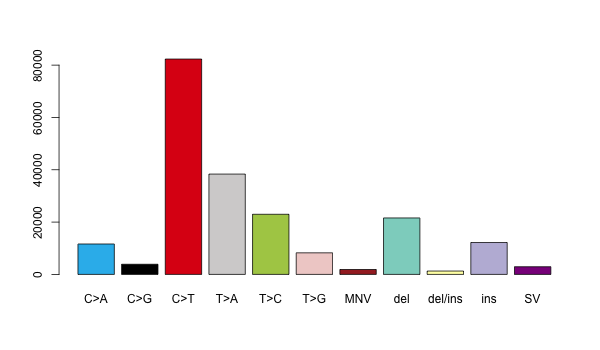
\includegraphics[scale = 0.6]{figures/Numbers_of_mutations.png}}
  \caption{Overall distribution of mutations across all samples after filtering. MNV: multi-nucleotide variants, del - deletion, ins - insertion, SV - structural variants.}
  \label{mut_distr}
\end{figure}

\end{document}